\subsection{Torque and change in angular momentum}
\paragraph{} $$\frac{dK}{dt}  = \frac{d}{dt}\left( \frac{1}{2}I\omega^2 \right) \stackrel{\parbox{1cm}{\centering \scriptsize I = const}}{=} \frac{1}{2}I\frac{d}{dt}\omega^2 = \frac{1}{2} \cdot I \left(\dot{\vec{\omega}}\vec{\omega} + \vec{\omega}\dot{\vec{\omega}}\right) = I\dot{\vec{\omega}} \vec{\omega} = \vec{N} \cdot \vec{\omega} $$


\begin{center}
	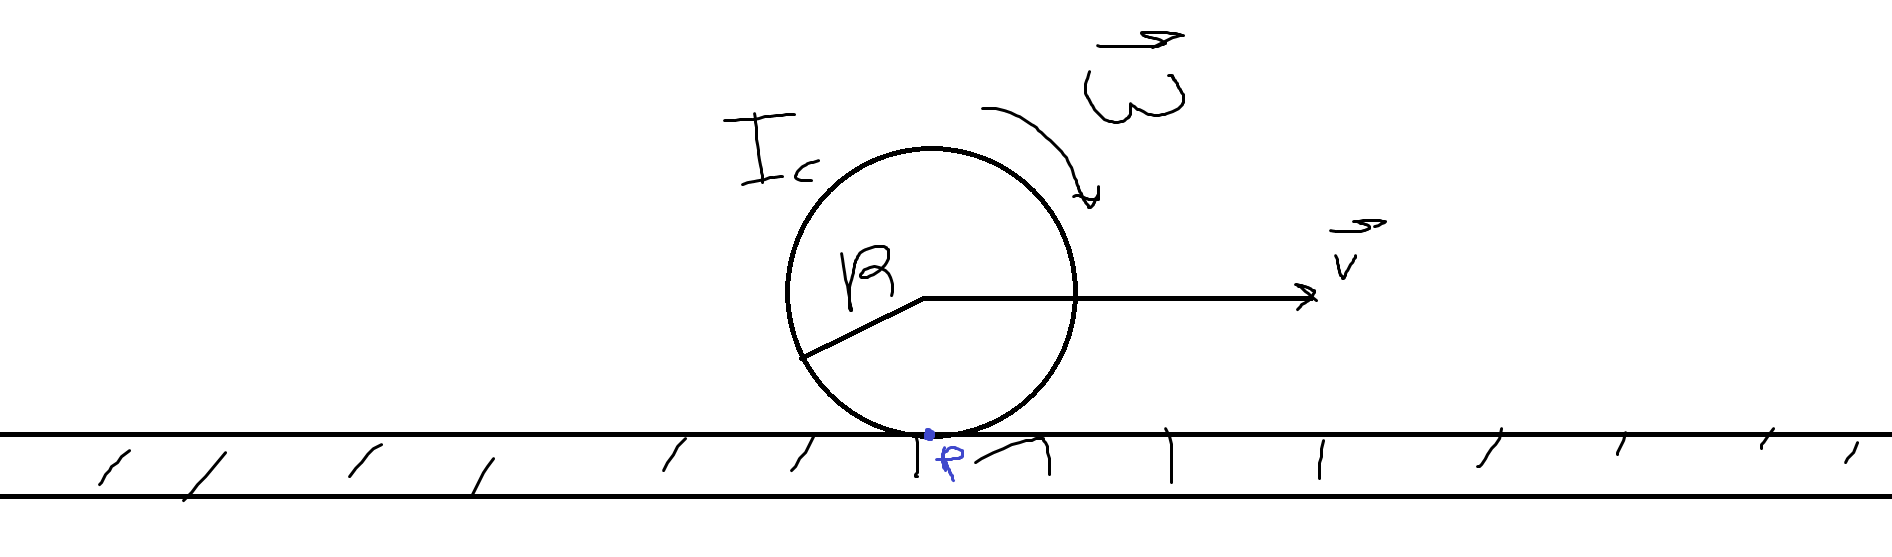
\includegraphics[width=\linewidth]{./lect18/pic1.png}
\end{center}
In point of contact $p$ there is no relative motion of body and a surface so there is only \textbf{static friction}. The condition for full rolling:
$$\omega R = v_c$$

In a given moment the body rotates around point $p$ with angular velocity $\omega$.


\begin{center}
	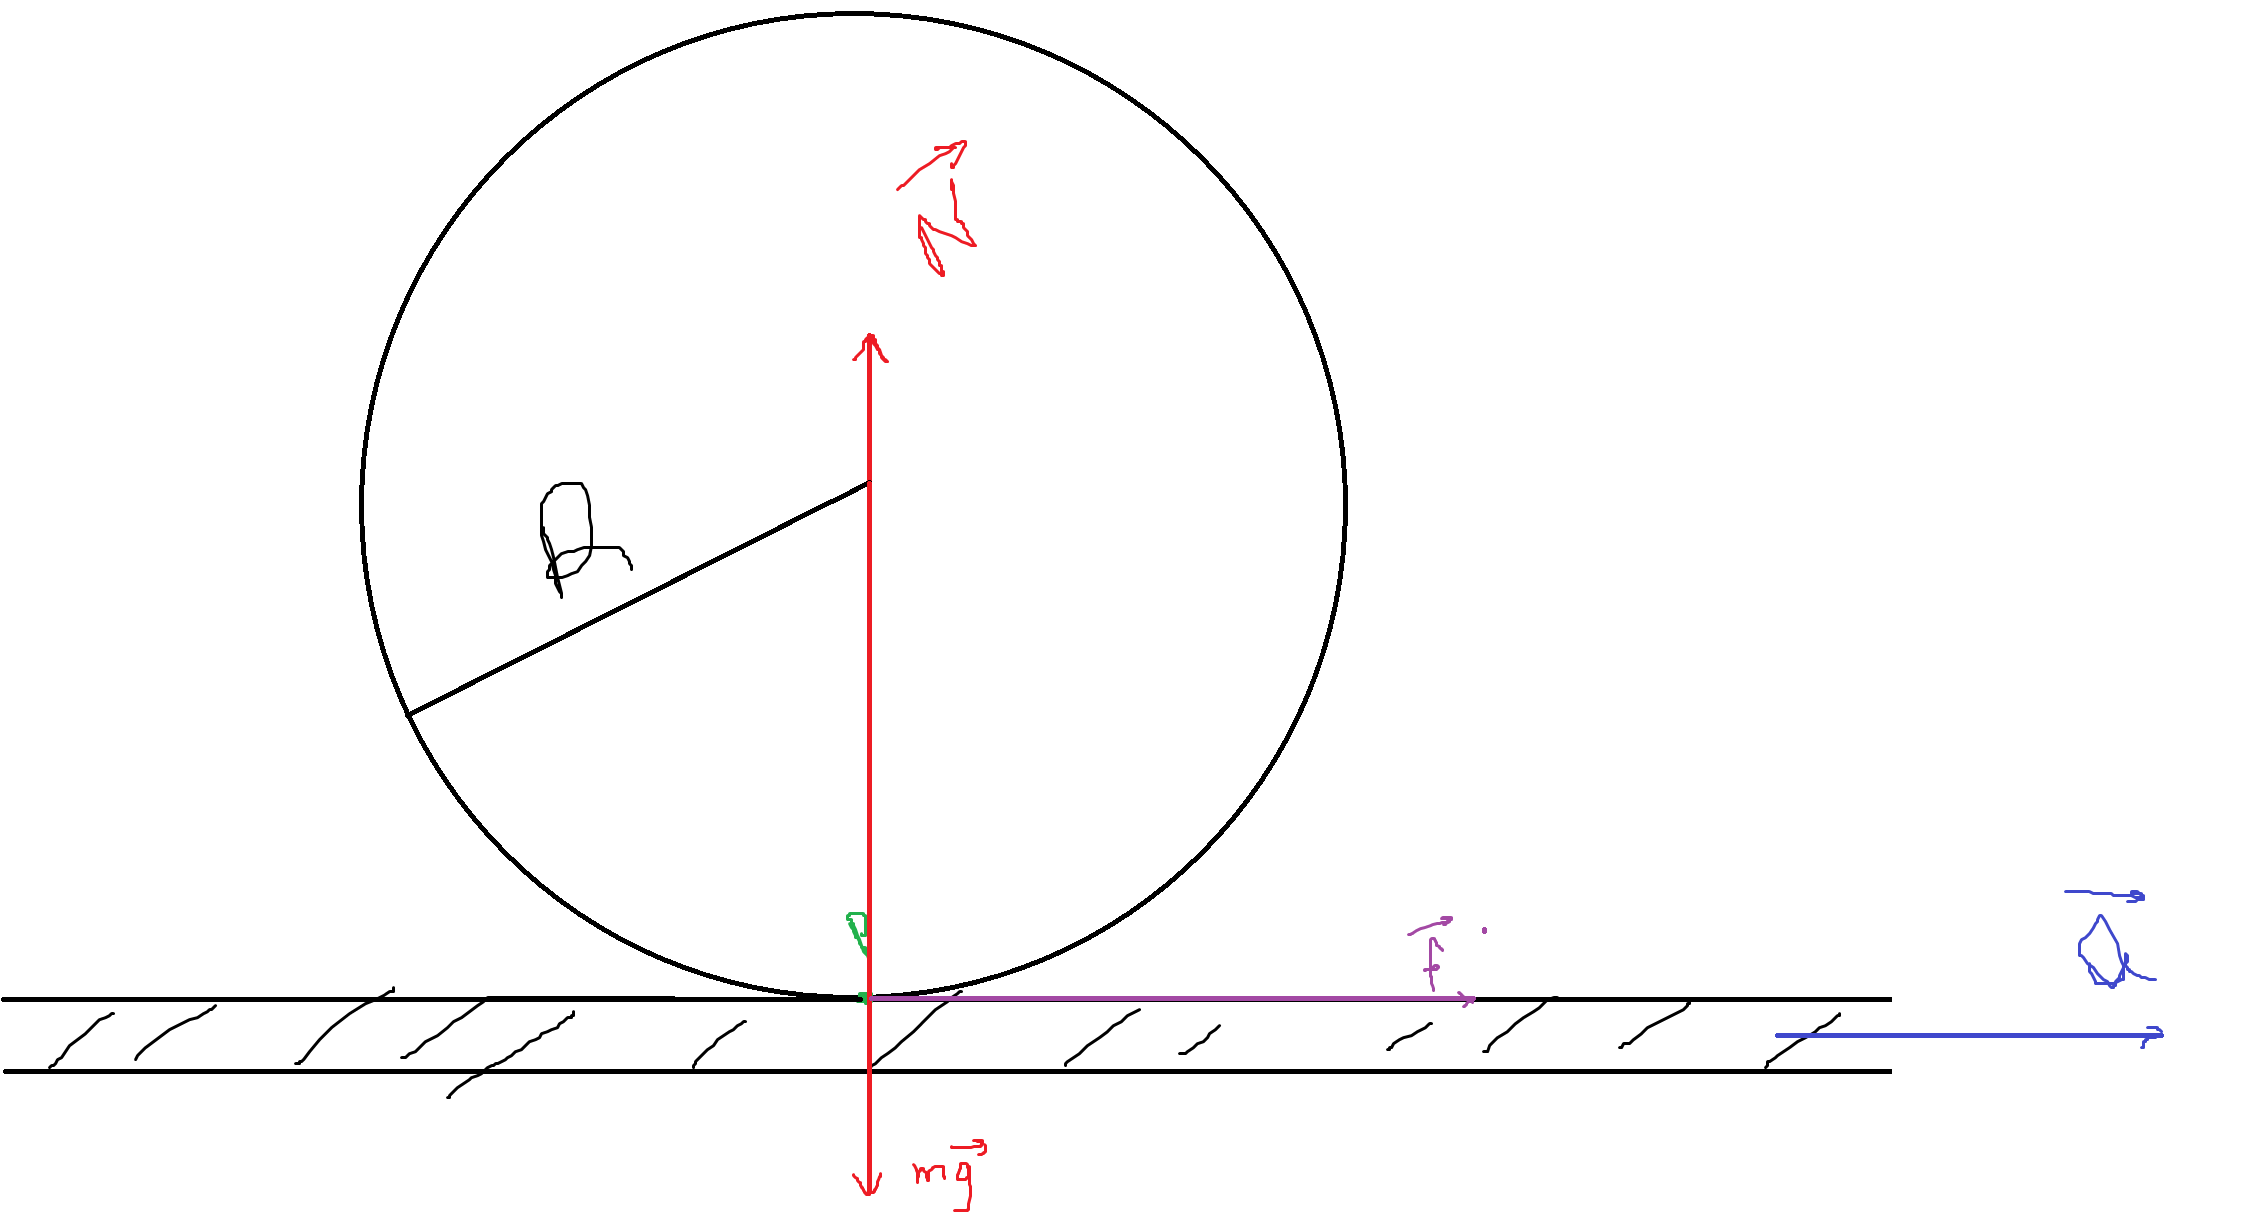
\includegraphics[width=\linewidth]{./lect18/pic2.png}
\end{center}
 
 
There is no moments for these forces:

$$\vec{N}_N = 0$$
$$\vec{N}_{mg} = 0$$
$$\vec{N}_{f} = 0$$

But there is still rotation since point $p$ accelerates.

Lets work around center of mass:

$$M\frac{dv_c}{dt} = f$$

Since $f$ is the only force in $x$ direction. It's torque is
$$\vec{N}_{cf} = Rf$$.

Motion equation for rolling (i.e. $\frac{d\omega}{dt}$):

$$I_c\frac{d\omega}{dt} = RF$$

By substituting $I_c = \frac{1}{2}MR^2$ for full cylinder:
$$\frac{1}{2}MR^2 \frac{d\omega}{dt} = Rf$$
$$\dot{v}_c = \frac{1}{2}R\dot{\omega}$$

\begin{center}
	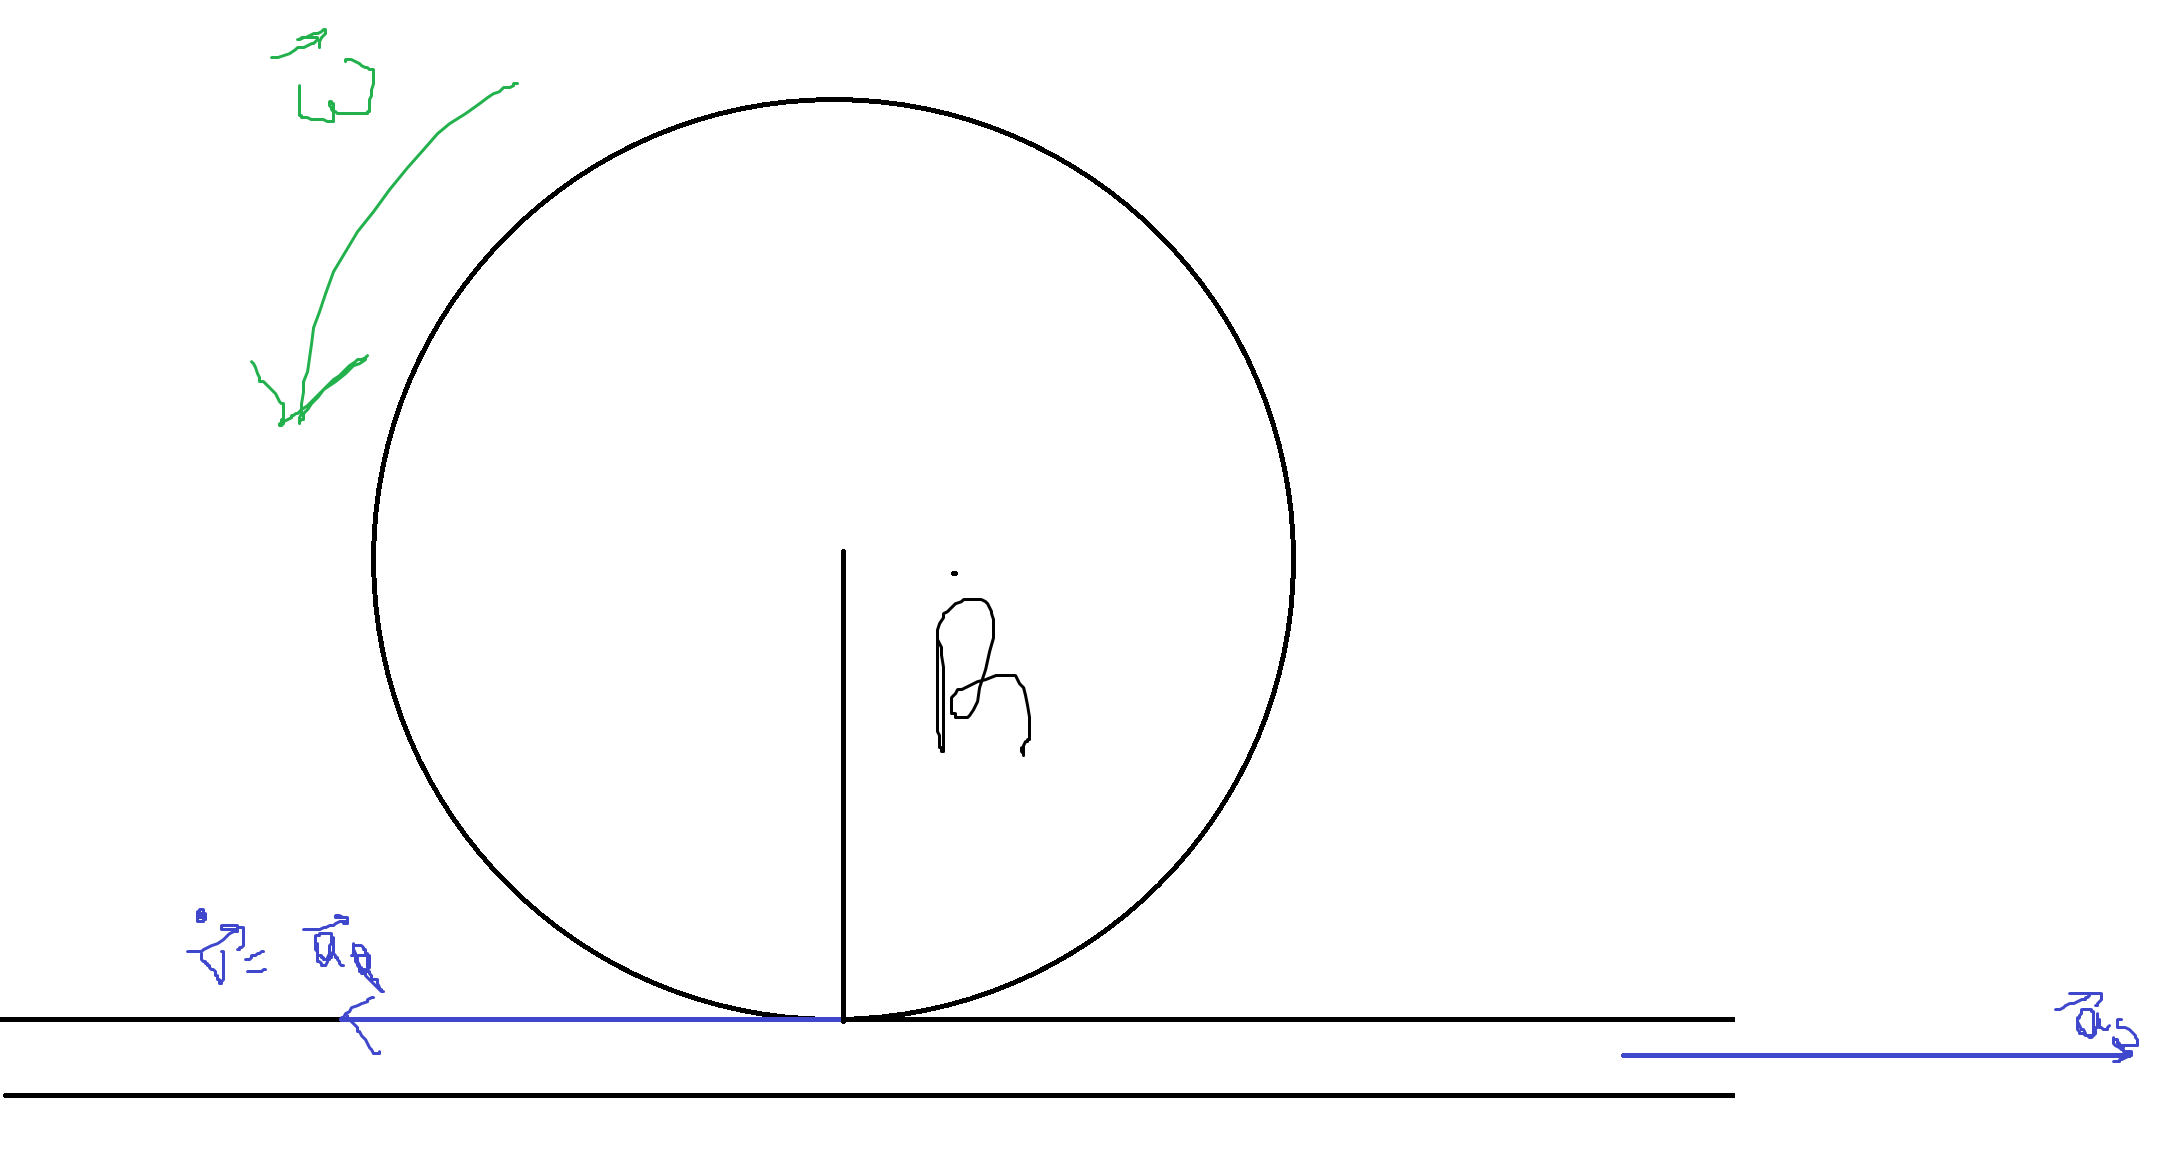
\includegraphics[width=\linewidth]{./lect18/pic3.png}
\end{center}

Surface acceleration is

$$a_s = a_p =\underbrace{ \frac{dv_c}{dt}}_{\parbox{2cm}{\centering \scriptsize acceleration due to motion}} + \underbrace{R\frac{d \omega}{dt}}_{\parbox{2cm}{\centering \scriptsize acceleration due to rotation}}$$

From

$$a = \frac{dv_c}{dt}+ R\frac{d\omega}{dt}$$

we get   $a_c = \dot{v}_c =\frac{1}{3}a$ and $f = \frac{1}{3}Ma$

\begin{center}
	\begin{tabular}{ccc}
		Value &	Linear&Angular \\
		Position&$\vec{r}$ & $\vec{\theta}$\\
		Velocity&$\vec{v} = \dot{\vec{r}}$ & $\vec{\omega}=\dot{\vec{\theta}}$\\
		Acceleration&$\vec{a} \ddot{\vec{r}}$ & $\vec{\alpha}= \ddot{\vec{\theta}}$\\
		Force&$\vec{F}$ & $\vec{N}$\\
		Mass&$M$ & $I$\\
		Momentum&$\vec{p}$ & $\vec{J}$\\
		Second law&$\vec{F} = m \vec{a}$ & $\vec{N} = I \vec{\alpha}$\\
		Kinetic energy&$K=\frac{mv^2}{2}$ & $K=\frac{I\omega^2}{2}$\\
		Work&$W = \int \vec{F} d\vec{x}$ & $W = \int \vec{N} d\vec{\theta}$\\
		Impulse&$\int \vec{F} dt$ & $\int \vec{N} dt$\\
		Power&$\vec{F} \cdot \vec{v}$ & $\vec{N} \cdot \vec{\omega}$
	\end{tabular}
\end{center}

\section{Harmonic oscillator}

Cyclic motion in non-closed trajectory.

\subsection{Spring}


\begin{center}
	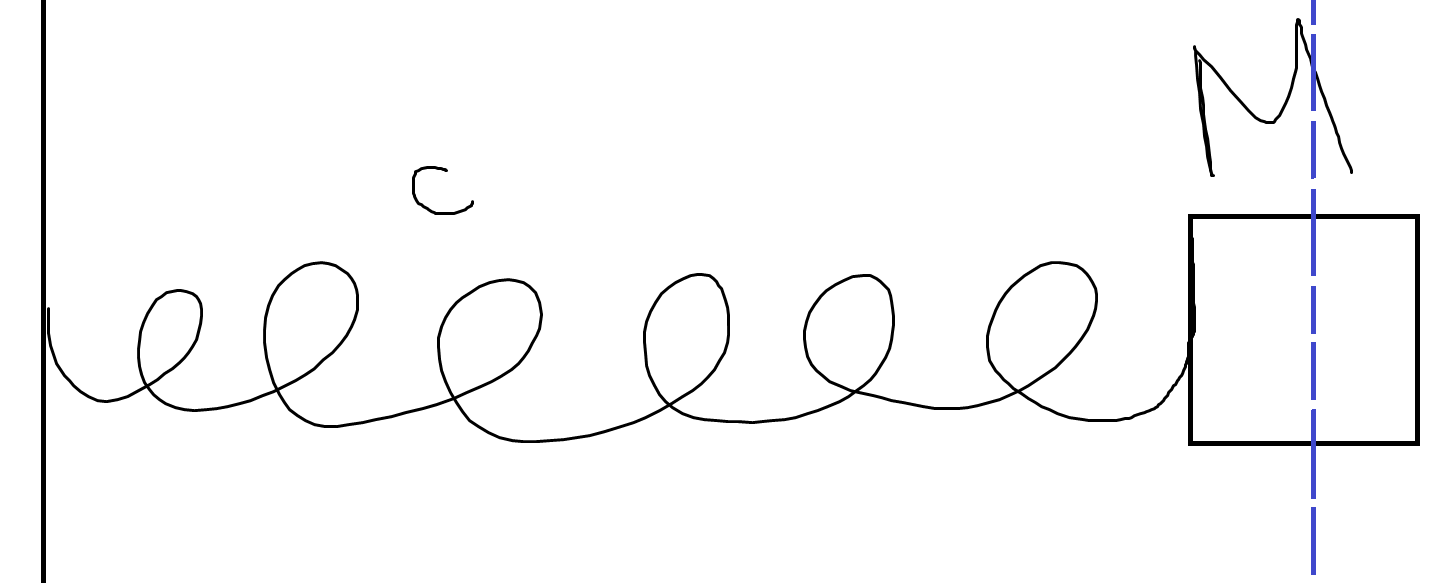
\includegraphics[width=\linewidth]{./lect18/pic4.png}
\end{center}

$x\hat{x}$ distance from equilibrium and $C$ is spring constant. Force acting on body is:

$$F = - Cx\hat{x}$$

From second law motion equation is: 
$$M\ddot{x} = - Cx$$

General solution is

$$x = A \sin\left(\omega_0 t + \phi \right) = A \cos\left(\omega_0 t + \phi - \frac{\pi}{2} \right)$$
or

$$x = B \sin \omega_0 t + D \sin \omega_0 t$$

$A=\sqrt{B^2+D^2}$ is amplitude. The solution is

$$\dot{x} = \frac{d}{dt} \left[ A \sin \left( \omega_0 t  +\phi \right) \right] = A\omega_0 \cos  \left( \omega_0 t  +\phi \right)$$
$$\ddot{x}  = \frac{d}{dt} \left[ A\omega_0 \cos  \left( \omega_0 t  +\phi \right) \right] = -\omega_0^2 x$$

By substituting:

$$M\left( \omega_0^2 x \right) - Cx$$

Acquiring $\omega_0$;

$$\omega_0 = \sqrt{\frac{C}{M}}$$ 

\paragraph{Note} $\omega_0 = \left[ \frac{rad}{s} \right]$, while number of cycles per second is $f_0 = \frac{\omega_0}{2\pi}$ and cycle time is $T = \frac{1}{f_0}$.

\paragraph{Energy conservation} Potential energy is $U = \frac{1}{2}Cx^2$. In regular problems this is a potential energy around equilibrium.

Total energy is:

$$E = \frac{1}{2}mv^2  + \frac{1}{2}cx^2$$

By deriving:

$$ 0 = mv\dot{v} + cx\dot{x} $$

which is the same equation by reduction of $\dot{x}$.

Another way to get it is to take energy when $x=0$:

$$\frac{1}{2}mv^2 = \frac{1}{2}CA^2 - \frac{1}{2}cx^2$$

$$v= \frac{dx}{dt} = \sqrt{\frac{C}{m}} \sqrt{A^2 - x^2}$$

$$\frac{dx}{\sqrt{A^2-x^2}} = \omega_0 dt$$

It can solved by integration and the solution of this equation is just same. 

\subsection{Damped Harmonic Oscillator}

in addition to returning force there is damping force $f=-bv$, where $v = -\dot{x}$ and $b$ is constant. Damping force coverts kinetic energy to heat (or something else) while returning force converts kinetic energy to potential and back. From second law:
$$m\ddot{x} = -Cx-d\dot{x}$$

Define $\tau = \frac{m}{b} [s]$ or $\frac{1}{\tau} = \frac{b}{m}$. Also $\omega_0^2 = \frac{C}{m}$. By dividing by $m$:

$$\ddot{x} + \frac{1}{\tau}\dot{x} + \omega_0^2x = 0$$

We acquired homogeneous linear differential equation with solution:

$$x=x_0e^{-\frac{t}{2\tau}}\sin\left( \omega_d t + \phi \right)$$

where $\phi$ and $x_0$ are initial conditions and

$$\omega_d = \left[ w_0^2 - \frac{1}{\left( 2\tau \right)^2} \right]^{\frac{1}{2}}$$

If $\omega_0^2 < \frac{1}{\left( 2 \tau \right)^2}$, then there is no oscillation.


\begin{center}
	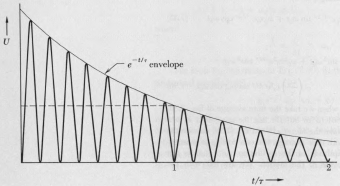
\includegraphics[width=\linewidth]{./lect18/pic5.png}
\end{center}